% Options for packages loaded elsewhere
\PassOptionsToPackage{unicode}{hyperref}
\PassOptionsToPackage{hyphens}{url}
\PassOptionsToPackage{dvipsnames,svgnames,x11names}{xcolor}
%
\documentclass[
  letterpaper,
  DIV=11,
  numbers=noendperiod]{scrartcl}

\usepackage{amsmath,amssymb}
\usepackage{iftex}
\ifPDFTeX
  \usepackage[T1]{fontenc}
  \usepackage[utf8]{inputenc}
  \usepackage{textcomp} % provide euro and other symbols
\else % if luatex or xetex
  \usepackage{unicode-math}
  \defaultfontfeatures{Scale=MatchLowercase}
  \defaultfontfeatures[\rmfamily]{Ligatures=TeX,Scale=1}
\fi
\usepackage{lmodern}
\ifPDFTeX\else  
    % xetex/luatex font selection
\fi
% Use upquote if available, for straight quotes in verbatim environments
\IfFileExists{upquote.sty}{\usepackage{upquote}}{}
\IfFileExists{microtype.sty}{% use microtype if available
  \usepackage[]{microtype}
  \UseMicrotypeSet[protrusion]{basicmath} % disable protrusion for tt fonts
}{}
\makeatletter
\@ifundefined{KOMAClassName}{% if non-KOMA class
  \IfFileExists{parskip.sty}{%
    \usepackage{parskip}
  }{% else
    \setlength{\parindent}{0pt}
    \setlength{\parskip}{6pt plus 2pt minus 1pt}}
}{% if KOMA class
  \KOMAoptions{parskip=half}}
\makeatother
\usepackage{xcolor}
\setlength{\emergencystretch}{3em} % prevent overfull lines
\setcounter{secnumdepth}{-\maxdimen} % remove section numbering
% Make \paragraph and \subparagraph free-standing
\makeatletter
\ifx\paragraph\undefined\else
  \let\oldparagraph\paragraph
  \renewcommand{\paragraph}{
    \@ifstar
      \xxxParagraphStar
      \xxxParagraphNoStar
  }
  \newcommand{\xxxParagraphStar}[1]{\oldparagraph*{#1}\mbox{}}
  \newcommand{\xxxParagraphNoStar}[1]{\oldparagraph{#1}\mbox{}}
\fi
\ifx\subparagraph\undefined\else
  \let\oldsubparagraph\subparagraph
  \renewcommand{\subparagraph}{
    \@ifstar
      \xxxSubParagraphStar
      \xxxSubParagraphNoStar
  }
  \newcommand{\xxxSubParagraphStar}[1]{\oldsubparagraph*{#1}\mbox{}}
  \newcommand{\xxxSubParagraphNoStar}[1]{\oldsubparagraph{#1}\mbox{}}
\fi
\makeatother

\usepackage{color}
\usepackage{fancyvrb}
\newcommand{\VerbBar}{|}
\newcommand{\VERB}{\Verb[commandchars=\\\{\}]}
\DefineVerbatimEnvironment{Highlighting}{Verbatim}{commandchars=\\\{\}}
% Add ',fontsize=\small' for more characters per line
\usepackage{framed}
\definecolor{shadecolor}{RGB}{241,243,245}
\newenvironment{Shaded}{\begin{snugshade}}{\end{snugshade}}
\newcommand{\AlertTok}[1]{\textcolor[rgb]{0.68,0.00,0.00}{#1}}
\newcommand{\AnnotationTok}[1]{\textcolor[rgb]{0.37,0.37,0.37}{#1}}
\newcommand{\AttributeTok}[1]{\textcolor[rgb]{0.40,0.45,0.13}{#1}}
\newcommand{\BaseNTok}[1]{\textcolor[rgb]{0.68,0.00,0.00}{#1}}
\newcommand{\BuiltInTok}[1]{\textcolor[rgb]{0.00,0.23,0.31}{#1}}
\newcommand{\CharTok}[1]{\textcolor[rgb]{0.13,0.47,0.30}{#1}}
\newcommand{\CommentTok}[1]{\textcolor[rgb]{0.37,0.37,0.37}{#1}}
\newcommand{\CommentVarTok}[1]{\textcolor[rgb]{0.37,0.37,0.37}{\textit{#1}}}
\newcommand{\ConstantTok}[1]{\textcolor[rgb]{0.56,0.35,0.01}{#1}}
\newcommand{\ControlFlowTok}[1]{\textcolor[rgb]{0.00,0.23,0.31}{\textbf{#1}}}
\newcommand{\DataTypeTok}[1]{\textcolor[rgb]{0.68,0.00,0.00}{#1}}
\newcommand{\DecValTok}[1]{\textcolor[rgb]{0.68,0.00,0.00}{#1}}
\newcommand{\DocumentationTok}[1]{\textcolor[rgb]{0.37,0.37,0.37}{\textit{#1}}}
\newcommand{\ErrorTok}[1]{\textcolor[rgb]{0.68,0.00,0.00}{#1}}
\newcommand{\ExtensionTok}[1]{\textcolor[rgb]{0.00,0.23,0.31}{#1}}
\newcommand{\FloatTok}[1]{\textcolor[rgb]{0.68,0.00,0.00}{#1}}
\newcommand{\FunctionTok}[1]{\textcolor[rgb]{0.28,0.35,0.67}{#1}}
\newcommand{\ImportTok}[1]{\textcolor[rgb]{0.00,0.46,0.62}{#1}}
\newcommand{\InformationTok}[1]{\textcolor[rgb]{0.37,0.37,0.37}{#1}}
\newcommand{\KeywordTok}[1]{\textcolor[rgb]{0.00,0.23,0.31}{\textbf{#1}}}
\newcommand{\NormalTok}[1]{\textcolor[rgb]{0.00,0.23,0.31}{#1}}
\newcommand{\OperatorTok}[1]{\textcolor[rgb]{0.37,0.37,0.37}{#1}}
\newcommand{\OtherTok}[1]{\textcolor[rgb]{0.00,0.23,0.31}{#1}}
\newcommand{\PreprocessorTok}[1]{\textcolor[rgb]{0.68,0.00,0.00}{#1}}
\newcommand{\RegionMarkerTok}[1]{\textcolor[rgb]{0.00,0.23,0.31}{#1}}
\newcommand{\SpecialCharTok}[1]{\textcolor[rgb]{0.37,0.37,0.37}{#1}}
\newcommand{\SpecialStringTok}[1]{\textcolor[rgb]{0.13,0.47,0.30}{#1}}
\newcommand{\StringTok}[1]{\textcolor[rgb]{0.13,0.47,0.30}{#1}}
\newcommand{\VariableTok}[1]{\textcolor[rgb]{0.07,0.07,0.07}{#1}}
\newcommand{\VerbatimStringTok}[1]{\textcolor[rgb]{0.13,0.47,0.30}{#1}}
\newcommand{\WarningTok}[1]{\textcolor[rgb]{0.37,0.37,0.37}{\textit{#1}}}

\providecommand{\tightlist}{%
  \setlength{\itemsep}{0pt}\setlength{\parskip}{0pt}}\usepackage{longtable,booktabs,array}
\usepackage{calc} % for calculating minipage widths
% Correct order of tables after \paragraph or \subparagraph
\usepackage{etoolbox}
\makeatletter
\patchcmd\longtable{\par}{\if@noskipsec\mbox{}\fi\par}{}{}
\makeatother
% Allow footnotes in longtable head/foot
\IfFileExists{footnotehyper.sty}{\usepackage{footnotehyper}}{\usepackage{footnote}}
\makesavenoteenv{longtable}
\usepackage{graphicx}
\makeatletter
\def\maxwidth{\ifdim\Gin@nat@width>\linewidth\linewidth\else\Gin@nat@width\fi}
\def\maxheight{\ifdim\Gin@nat@height>\textheight\textheight\else\Gin@nat@height\fi}
\makeatother
% Scale images if necessary, so that they will not overflow the page
% margins by default, and it is still possible to overwrite the defaults
% using explicit options in \includegraphics[width, height, ...]{}
\setkeys{Gin}{width=\maxwidth,height=\maxheight,keepaspectratio}
% Set default figure placement to htbp
\makeatletter
\def\fps@figure{htbp}
\makeatother

\KOMAoption{captions}{tableheading}
\makeatletter
\@ifpackageloaded{caption}{}{\usepackage{caption}}
\AtBeginDocument{%
\ifdefined\contentsname
  \renewcommand*\contentsname{Table of contents}
\else
  \newcommand\contentsname{Table of contents}
\fi
\ifdefined\listfigurename
  \renewcommand*\listfigurename{List of Figures}
\else
  \newcommand\listfigurename{List of Figures}
\fi
\ifdefined\listtablename
  \renewcommand*\listtablename{List of Tables}
\else
  \newcommand\listtablename{List of Tables}
\fi
\ifdefined\figurename
  \renewcommand*\figurename{Figure}
\else
  \newcommand\figurename{Figure}
\fi
\ifdefined\tablename
  \renewcommand*\tablename{Table}
\else
  \newcommand\tablename{Table}
\fi
}
\@ifpackageloaded{float}{}{\usepackage{float}}
\floatstyle{ruled}
\@ifundefined{c@chapter}{\newfloat{codelisting}{h}{lop}}{\newfloat{codelisting}{h}{lop}[chapter]}
\floatname{codelisting}{Listing}
\newcommand*\listoflistings{\listof{codelisting}{List of Listings}}
\makeatother
\makeatletter
\makeatother
\makeatletter
\@ifpackageloaded{caption}{}{\usepackage{caption}}
\@ifpackageloaded{subcaption}{}{\usepackage{subcaption}}
\makeatother
\ifLuaTeX
  \usepackage{selnolig}  % disable illegal ligatures
\fi
\usepackage{bookmark}

\IfFileExists{xurl.sty}{\usepackage{xurl}}{} % add URL line breaks if available
\urlstyle{same} % disable monospaced font for URLs
\hypersetup{
  pdftitle={Métodos numéricos Tarea 10},
  colorlinks=true,
  linkcolor={blue},
  filecolor={Maroon},
  citecolor={Blue},
  urlcolor={Blue},
  pdfcreator={LaTeX via pandoc}}

\title{Métodos numéricos Tarea 10}
\author{}
\date{}

\begin{document}
\maketitle

\href{https://github.com/Bidobelemti/M-todos-num-ricos/tree/main}{Enlace
a repositorio}

https://github.com/Bidobelemti/M-todos-num-ricos/tree/main

\begin{enumerate}
\def\labelenumi{\arabic{enumi}.}
\tightlist
\item
  Realice las siguientes multiplicaciones matriz - matriz
\end{enumerate}

\begin{Shaded}
\begin{Highlighting}[]
\ImportTok{import}\NormalTok{ numpy }\ImportTok{as}\NormalTok{ np}
\NormalTok{A }\OperatorTok{=}\NormalTok{ [}
\NormalTok{    [}\DecValTok{2}\NormalTok{,}\OperatorTok{{-}}\DecValTok{3}\NormalTok{],}
\NormalTok{    [}\DecValTok{3}\NormalTok{,}\OperatorTok{{-}}\DecValTok{1}\NormalTok{]]}
\NormalTok{B }\OperatorTok{=}\NormalTok{ [}
\NormalTok{    [}\DecValTok{1}\NormalTok{,}\DecValTok{5}\NormalTok{],}
\NormalTok{    [}\DecValTok{2}\NormalTok{,}\DecValTok{0}\NormalTok{]]}
\NormalTok{np.dot(np.array(A), np.array(B))}
\end{Highlighting}
\end{Shaded}

\begin{verbatim}
array([[-4, 10],
       [ 1, 15]])
\end{verbatim}

\begin{Shaded}
\begin{Highlighting}[]
\NormalTok{A1 }\OperatorTok{=}\NormalTok{ [}
\NormalTok{    [}\DecValTok{2}\NormalTok{,}\OperatorTok{{-}}\DecValTok{3}\NormalTok{],}
\NormalTok{    [}\DecValTok{3}\NormalTok{,}\OperatorTok{{-}}\DecValTok{1}\NormalTok{]}
\NormalTok{]}

\NormalTok{B1 }\OperatorTok{=}\NormalTok{ [}
\NormalTok{    [}\DecValTok{1}\NormalTok{,}\DecValTok{5}\NormalTok{,}\OperatorTok{{-}}\DecValTok{4}\NormalTok{],}
\NormalTok{    [}\OperatorTok{{-}}\DecValTok{3}\NormalTok{,}\DecValTok{2}\NormalTok{,}\DecValTok{0}\NormalTok{]}
\NormalTok{]}
\NormalTok{np.dot(np.array(A1), np.array(B1))}
\end{Highlighting}
\end{Shaded}

\begin{verbatim}
array([[ 11,   4,  -8],
       [  6,  13, -12]])
\end{verbatim}

\begin{Shaded}
\begin{Highlighting}[]
\NormalTok{A2 }\OperatorTok{=}\NormalTok{ [}
\NormalTok{    [}\DecValTok{2}\NormalTok{,}\OperatorTok{{-}}\DecValTok{3}\NormalTok{,}\DecValTok{1}\NormalTok{],}
\NormalTok{    [}\DecValTok{4}\NormalTok{,}\DecValTok{3}\NormalTok{,}\DecValTok{0}\NormalTok{],}
\NormalTok{    [}\DecValTok{5}\NormalTok{,}\DecValTok{2}\NormalTok{,}\OperatorTok{{-}}\DecValTok{4}\NormalTok{]}
\NormalTok{]}

\NormalTok{B2 }\OperatorTok{=}\NormalTok{ [}
\NormalTok{    [}\DecValTok{0}\NormalTok{,}\DecValTok{1}\NormalTok{,}\OperatorTok{{-}}\DecValTok{2}\NormalTok{],}
\NormalTok{    [}\DecValTok{1}\NormalTok{,}\DecValTok{0}\NormalTok{,}\OperatorTok{{-}}\DecValTok{1}\NormalTok{],}
\NormalTok{    [}\DecValTok{2}\NormalTok{,}\DecValTok{3}\NormalTok{,}\OperatorTok{{-}}\DecValTok{2}\NormalTok{]}
\NormalTok{]}
\NormalTok{np.dot(np.array(A2), np.array(B2))}
\end{Highlighting}
\end{Shaded}

\begin{verbatim}
array([[ -1,   5,  -3],
       [  3,   4, -11],
       [ -6,  -7,  -4]])
\end{verbatim}

\begin{Shaded}
\begin{Highlighting}[]
\NormalTok{A3 }\OperatorTok{=}\NormalTok{ [}
\NormalTok{    [}\DecValTok{2}\NormalTok{,}\DecValTok{1}\NormalTok{,}\DecValTok{2}\NormalTok{],}
\NormalTok{    [}\OperatorTok{{-}}\DecValTok{2}\NormalTok{,}\DecValTok{3}\NormalTok{,}\DecValTok{0}\NormalTok{],}
\NormalTok{    [}\DecValTok{2}\NormalTok{,}\OperatorTok{{-}}\DecValTok{1}\NormalTok{,}\DecValTok{3}\NormalTok{]}
\NormalTok{]}

\NormalTok{B3 }\OperatorTok{=}\NormalTok{ [}
\NormalTok{    [}\DecValTok{1}\NormalTok{,}\OperatorTok{{-}}\DecValTok{2}\NormalTok{],}
\NormalTok{    [}\OperatorTok{{-}}\DecValTok{4}\NormalTok{,}\DecValTok{1}\NormalTok{],}
\NormalTok{    [}\DecValTok{0}\NormalTok{,}\DecValTok{2}\NormalTok{]}
\NormalTok{]}
\NormalTok{np.dot(np.array(A3), np.array(B3))}
\end{Highlighting}
\end{Shaded}

\begin{verbatim}
array([[ -2,   1],
       [-14,   7],
       [  6,   1]])
\end{verbatim}

\begin{enumerate}
\def\labelenumi{\arabic{enumi}.}
\setcounter{enumi}{1}
\tightlist
\item
  Determine cualés de las siguientes matrices son no singulares y
  calcule la inversa de esas matrices.
\end{enumerate}

\begin{Shaded}
\begin{Highlighting}[]
\CommentTok{\# matriz singular aquella que su determinante es 0}
\ImportTok{from}\NormalTok{ src }\ImportTok{import}\NormalTok{ calc\_determinante}

\NormalTok{A }\OperatorTok{=}\NormalTok{ [}
\NormalTok{    [}\DecValTok{4}\NormalTok{,}\DecValTok{2}\NormalTok{,}\DecValTok{6}\NormalTok{],}
\NormalTok{    [}\DecValTok{3}\NormalTok{,}\DecValTok{0}\NormalTok{,}\DecValTok{7}\NormalTok{],}
\NormalTok{    [}\OperatorTok{{-}}\DecValTok{2}\NormalTok{,}\OperatorTok{{-}}\DecValTok{1}\NormalTok{,}\OperatorTok{{-}}\DecValTok{3}\NormalTok{]}
\NormalTok{]}

\NormalTok{calc\_determinante(A)}
\end{Highlighting}
\end{Shaded}

\begin{verbatim}
ValueError: No existe solución única.
---------------------------------------------------------------------------
ValueError                                Traceback (most recent call last)
Cell In[10], line 10
      2 from src import calc_determinante
      4 A = [
      5     [4,2,6],
      6     [3,0,7],
      7     [-2,-1,-3]
      8 ]
---> 10 calc_determinante(A)

File c:\Users\mauri\OneDrive\Documentos\Universidad\2024a\Metodos\metodos git\M-todos-num-ricos\Tarea10_MN\src\funciones.py:160, in calc_determinante(A)
    149 """Función que calcula el determinante usando el método
    150 [Descomposición LU, eliminación gaussiana, Gauss-Jordan, Gauss-Jacobi o Gauss-Seidel]
    151 
   (...)
    157 
    158 """
    159     # Descomposición LU
--> 160 L, U = descomposicion_LU(A)
    162 # El determinante es el producto de los elementos diagonales de U
    163 det_U = 1

File c:\Users\mauri\OneDrive\Documentos\Universidad\2024a\Metodos\metodos git\M-todos-num-ricos\Tarea10_MN\src\funciones.py:34, in descomposicion_LU(A)
     30 for i in range(0, n):  # loop por columna
     31 
     32     # --- deterimnar pivote
     33     if A[i, i] == 0:
---> 34         raise ValueError("No existe solución única.")
     36     # --- Eliminación: loop por fila
     37     L[i, i] = 1

ValueError: No existe solución única.
\end{verbatim}

Dado que menciona que no posee solución única es indicativo que su
determinante es 0, por lo tanto no existe inversa de dicha matriz.

\begin{Shaded}
\begin{Highlighting}[]
\NormalTok{B}\OperatorTok{=}\NormalTok{[}
\NormalTok{    [}\DecValTok{1}\NormalTok{,}\DecValTok{2}\NormalTok{,}\DecValTok{0}\NormalTok{],}
\NormalTok{    [}\DecValTok{2}\NormalTok{,}\DecValTok{1}\NormalTok{,}\OperatorTok{{-}}\DecValTok{1}\NormalTok{],}
\NormalTok{    [}\DecValTok{3}\NormalTok{,}\DecValTok{1}\NormalTok{,}\DecValTok{1}\NormalTok{]}
\NormalTok{]}

\BuiltInTok{print}\NormalTok{(}\SpecialStringTok{f\textquotesingle{}la determinante es: }\SpecialCharTok{\{}\NormalTok{calc\_determinante(B)}\SpecialCharTok{\}}\SpecialStringTok{\textquotesingle{}}\NormalTok{)}
\NormalTok{inv\_B }\OperatorTok{=}\NormalTok{ np.linalg.inv(np.array(B))}
\BuiltInTok{print}\NormalTok{(inv\_B)}
\end{Highlighting}
\end{Shaded}

\begin{verbatim}
la determinante es: -8.0
[[-0.25   0.25   0.25 ]
 [ 0.625 -0.125 -0.125]
 [ 0.125 -0.625  0.375]]
\end{verbatim}

\begin{Shaded}
\begin{Highlighting}[]
\NormalTok{C}\OperatorTok{=}\NormalTok{[}
\NormalTok{    [}\DecValTok{1}\NormalTok{,}\DecValTok{1}\NormalTok{,}\OperatorTok{{-}}\DecValTok{1}\NormalTok{,}\DecValTok{1}\NormalTok{],}
\NormalTok{    [}\DecValTok{1}\NormalTok{,}\DecValTok{2}\NormalTok{,}\OperatorTok{{-}}\DecValTok{4}\NormalTok{,}\OperatorTok{{-}}\DecValTok{2}\NormalTok{],}
\NormalTok{    [}\DecValTok{2}\NormalTok{,}\DecValTok{1}\NormalTok{,}\DecValTok{1}\NormalTok{,}\DecValTok{5}\NormalTok{],}
\NormalTok{    [}\OperatorTok{{-}}\DecValTok{1}\NormalTok{,}\DecValTok{0}\NormalTok{,}\OperatorTok{{-}}\DecValTok{2}\NormalTok{,}\OperatorTok{{-}}\DecValTok{4}\NormalTok{]}
\NormalTok{]}

\BuiltInTok{print}\NormalTok{(}\SpecialStringTok{f\textquotesingle{}la determinante es: }\SpecialCharTok{\{}\NormalTok{calc\_determinante(C)}\SpecialCharTok{\}}\SpecialStringTok{\textquotesingle{}}\NormalTok{)}
\end{Highlighting}
\end{Shaded}

\begin{verbatim}
ValueError: No existe solución única.
---------------------------------------------------------------------------
ValueError                                Traceback (most recent call last)
Cell In[16], line 8
      1 C=[
      2     [1,1,-1,1],
      3     [1,2,-4,-2],
      4     [2,1,1,5],
      5     [-1,0,-2,-4]
      6 ]
----> 8 print(f'la determinante es: {calc_determinante(C)}')
      9 inv_B = np.linalg.inv(np.array(B))

File c:\Users\mauri\OneDrive\Documentos\Universidad\2024a\Metodos\metodos git\M-todos-num-ricos\Tarea10_MN\src\funciones.py:160, in calc_determinante(A)
    149 """Función que calcula el determinante usando el método
    150 [Descomposición LU, eliminación gaussiana, Gauss-Jordan, Gauss-Jacobi o Gauss-Seidel]
    151 
   (...)
    157 
    158 """
    159     # Descomposición LU
--> 160 L, U = descomposicion_LU(A)
    162 # El determinante es el producto de los elementos diagonales de U
    163 det_U = 1

File c:\Users\mauri\OneDrive\Documentos\Universidad\2024a\Metodos\metodos git\M-todos-num-ricos\Tarea10_MN\src\funciones.py:34, in descomposicion_LU(A)
     30 for i in range(0, n):  # loop por columna
     31 
     32     # --- deterimnar pivote
     33     if A[i, i] == 0:
---> 34         raise ValueError("No existe solución única.")
     36     # --- Eliminación: loop por fila
     37     L[i, i] = 1

ValueError: No existe solución única.
\end{verbatim}

\begin{Shaded}
\begin{Highlighting}[]
\NormalTok{D }\OperatorTok{=}\NormalTok{ [}
\NormalTok{    [}\DecValTok{4}\NormalTok{, }\DecValTok{0}\NormalTok{, }\DecValTok{0}\NormalTok{, }\DecValTok{0}\NormalTok{],}
\NormalTok{    [}\DecValTok{6}\NormalTok{, }\DecValTok{7}\NormalTok{, }\DecValTok{0}\NormalTok{, }\DecValTok{0}\NormalTok{],}
\NormalTok{    [}\DecValTok{9}\NormalTok{, }\DecValTok{11}\NormalTok{, }\DecValTok{1}\NormalTok{, }\DecValTok{0}\NormalTok{],}
\NormalTok{    [}\DecValTok{5}\NormalTok{, }\DecValTok{4}\NormalTok{, }\DecValTok{1}\NormalTok{, }\DecValTok{1}\NormalTok{]}
\NormalTok{]}
\BuiltInTok{print}\NormalTok{(}\SpecialStringTok{f\textquotesingle{}la determinante es: }\SpecialCharTok{\{}\NormalTok{calc\_determinante(D)}\SpecialCharTok{\}}\SpecialStringTok{\textquotesingle{}}\NormalTok{)}
\NormalTok{inv\_D }\OperatorTok{=}\NormalTok{ np.linalg.inv(np.array(D))}
\BuiltInTok{print}\NormalTok{(inv\_D)}
\end{Highlighting}
\end{Shaded}

\begin{verbatim}
la determinante es: 28.0
[[ 2.50000000e-01  6.16790569e-18  0.00000000e+00  0.00000000e+00]
 [-2.14285714e-01  1.42857143e-01 -0.00000000e+00 -0.00000000e+00]
 [ 1.07142857e-01 -1.57142857e+00  1.00000000e+00 -0.00000000e+00]
 [-5.00000000e-01  1.00000000e+00 -1.00000000e+00  1.00000000e+00]]
\end{verbatim}

\begin{enumerate}
\def\labelenumi{\arabic{enumi}.}
\setcounter{enumi}{2}
\tightlist
\item
  Resuelva
\end{enumerate}

\(x_1 - x_2 + 2x_3 - x_4 = 6, x_1-x_3+x_4=4,2x_1+x_2+3x_3-4x_4=-2,-x_2+x_3-x_4=5\)

\(x_1 - x_2 + 2x_3 - x_4 = 1, x_1-x_3+x_4=1,2x_1+x_2+3x_3-4x_4=2,-x_2+x_3-x_4=1\)

\begin{Shaded}
\begin{Highlighting}[]
\ImportTok{from}\NormalTok{ src }\ImportTok{import}\NormalTok{ descomposicion\_LU, resolver\_LU}
\NormalTok{A }\OperatorTok{=}\NormalTok{ [}
\NormalTok{    [}\DecValTok{1}\NormalTok{,}\OperatorTok{{-}}\DecValTok{1}\NormalTok{,}\DecValTok{2}\NormalTok{,}\OperatorTok{{-}}\DecValTok{1}\NormalTok{],}
\NormalTok{    [}\DecValTok{1}\NormalTok{,}\DecValTok{0}\NormalTok{,}\OperatorTok{{-}}\DecValTok{1}\NormalTok{,}\DecValTok{1}\NormalTok{],}
\NormalTok{    [}\DecValTok{2}\NormalTok{,}\DecValTok{1}\NormalTok{,}\DecValTok{3}\NormalTok{,}\DecValTok{4}\NormalTok{],}
\NormalTok{    [}\DecValTok{0}\NormalTok{,}\OperatorTok{{-}}\DecValTok{1}\NormalTok{,}\DecValTok{1}\NormalTok{,}\OperatorTok{{-}}\DecValTok{1}\NormalTok{]}
\NormalTok{]}

\NormalTok{L,U }\OperatorTok{=}\NormalTok{ descomposicion\_LU(A)}

\NormalTok{b1 }\OperatorTok{=}\NormalTok{ [}\DecValTok{6}\NormalTok{,}\DecValTok{4}\NormalTok{,}\OperatorTok{{-}}\DecValTok{2}\NormalTok{,}\DecValTok{5}\NormalTok{]}
\NormalTok{b2 }\OperatorTok{=}\NormalTok{ [}\DecValTok{1}\NormalTok{,}\DecValTok{1}\NormalTok{,}\DecValTok{2}\NormalTok{,}\OperatorTok{{-}}\DecValTok{1}\NormalTok{]}

\NormalTok{answer\_one }\OperatorTok{=}\NormalTok{ resolver\_LU(L}\OperatorTok{=}\NormalTok{L, U}\OperatorTok{=}\NormalTok{U, b}\OperatorTok{=}\NormalTok{b1)}
\NormalTok{answer\_two }\OperatorTok{=}\NormalTok{ resolver\_LU(L}\OperatorTok{=}\NormalTok{L, U}\OperatorTok{=}\NormalTok{U, b}\OperatorTok{=}\NormalTok{b2)}

\BuiltInTok{print}\NormalTok{(}\SpecialStringTok{f\textquotesingle{}La primera respuesta es = }\SpecialCharTok{\{}\NormalTok{answer\_one}\SpecialCharTok{\}}\SpecialStringTok{\textquotesingle{}}\NormalTok{)}
\BuiltInTok{print}\NormalTok{(}\SpecialStringTok{f\textquotesingle{}La primera respuesta es = }\SpecialCharTok{\{}\NormalTok{answer\_two}\SpecialCharTok{\}}\SpecialStringTok{\textquotesingle{}}\NormalTok{)}
\end{Highlighting}
\end{Shaded}

\begin{verbatim}
La primera respuesta es = [[ 2.]
 [-7.]
 [-1.]
 [ 1.]]
La primera respuesta es = [[ 2.]
 [ 2.]
 [ 0.]
 [-1.]]
\end{verbatim}

\begin{enumerate}
\def\labelenumi{\arabic{enumi}.}
\setcounter{enumi}{3}
\tightlist
\item
  Encuentre los valores de A que hacen que la siguiente matriz sea
  singular. \[
  \begin{matrix}
  1 & -1 & \alpha \\
  2 & 2 & 1 \\
  0 & \alpha & -\frac{3}{2}
  \end{matrix}
  \]
\end{enumerate}

\begin{figure}[H]

{\centering 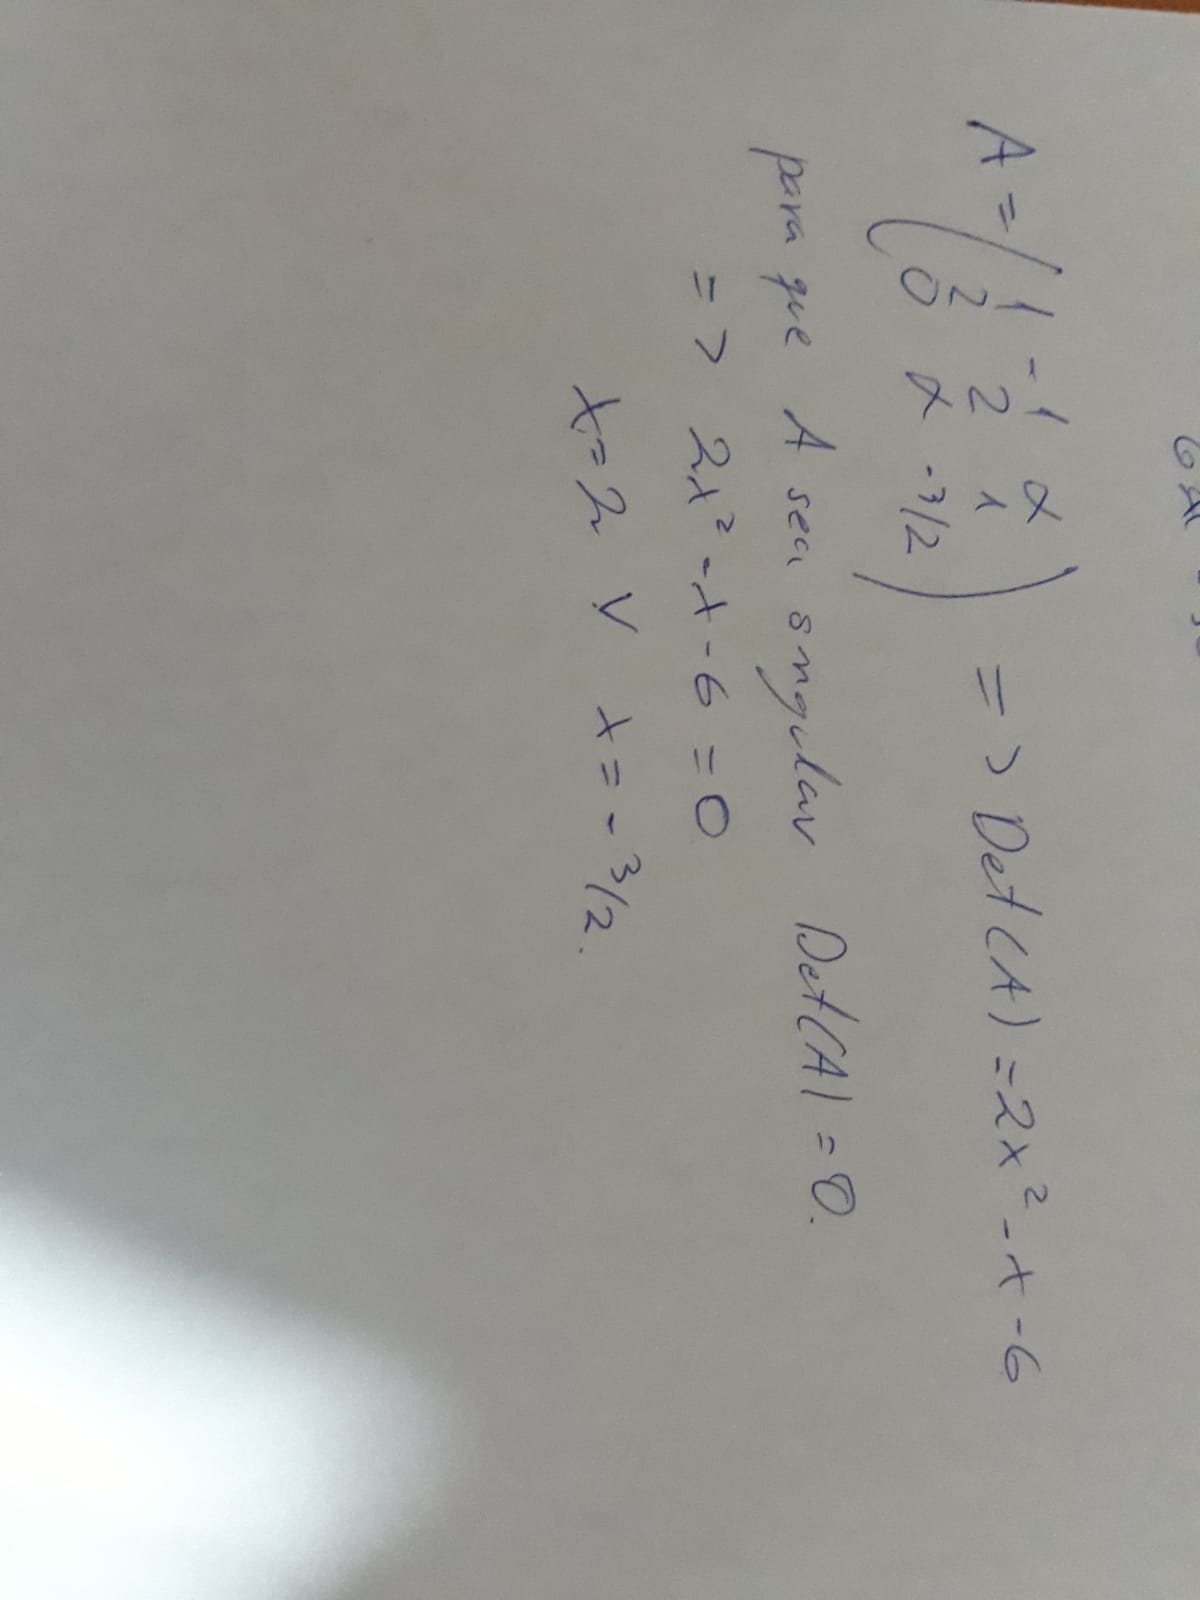
\includegraphics{images/image.jpeg}

}

\caption{Pregunta 4}

\end{figure}%

\begin{enumerate}
\def\labelenumi{\arabic{enumi}.}
\setcounter{enumi}{4}
\tightlist
\item
  Resuelva los siguientes sistemas lineales
\end{enumerate}

\begin{Shaded}
\begin{Highlighting}[]
\NormalTok{L }\OperatorTok{=}\NormalTok{ [}
\NormalTok{    [}\DecValTok{1}\NormalTok{, }\DecValTok{0}\NormalTok{, }\DecValTok{0}\NormalTok{],}
\NormalTok{    [}\DecValTok{2}\NormalTok{, }\DecValTok{1}\NormalTok{, }\DecValTok{0}\NormalTok{],}
\NormalTok{    [}\OperatorTok{{-}}\DecValTok{1}\NormalTok{, }\DecValTok{0}\NormalTok{, }\DecValTok{1}\NormalTok{]}
\NormalTok{]}

\NormalTok{U }\OperatorTok{=}\NormalTok{ [}
\NormalTok{    [}\DecValTok{2}\NormalTok{,}\DecValTok{3}\NormalTok{,}\OperatorTok{{-}}\DecValTok{1}\NormalTok{],}
\NormalTok{    [}\DecValTok{0}\NormalTok{,}\OperatorTok{{-}}\DecValTok{2}\NormalTok{,}\DecValTok{1}\NormalTok{],}
\NormalTok{    [}\DecValTok{0}\NormalTok{,}\DecValTok{0}\NormalTok{,}\DecValTok{3}\NormalTok{]}
\NormalTok{]}

\NormalTok{b }\OperatorTok{=}\NormalTok{ [}\DecValTok{2}\NormalTok{, }\OperatorTok{{-}}\DecValTok{1}\NormalTok{, }\DecValTok{1}\NormalTok{]}

\BuiltInTok{print}\NormalTok{(resolver\_LU(L}\OperatorTok{=}\NormalTok{np.array(L),U}\OperatorTok{=}\NormalTok{np.array(U),b}\OperatorTok{=}\NormalTok{b))}
\end{Highlighting}
\end{Shaded}

\begin{verbatim}
[[-3.]
 [ 3.]
 [ 1.]]
\end{verbatim}

\begin{Shaded}
\begin{Highlighting}[]
\NormalTok{L }\OperatorTok{=}\NormalTok{ [}
\NormalTok{    [}\DecValTok{2}\NormalTok{, }\DecValTok{0}\NormalTok{, }\DecValTok{0}\NormalTok{],}
\NormalTok{    [}\OperatorTok{{-}}\DecValTok{1}\NormalTok{, }\DecValTok{1}\NormalTok{, }\DecValTok{0}\NormalTok{],}
\NormalTok{    [}\DecValTok{3}\NormalTok{, }\DecValTok{2}\NormalTok{, }\OperatorTok{{-}}\DecValTok{1}\NormalTok{]}
\NormalTok{]}

\NormalTok{U }\OperatorTok{=}\NormalTok{ [}
\NormalTok{    [}\DecValTok{1}\NormalTok{,}\DecValTok{1}\NormalTok{,}\DecValTok{1}\NormalTok{],}
\NormalTok{    [}\DecValTok{0}\NormalTok{,}\DecValTok{1}\NormalTok{,}\DecValTok{2}\NormalTok{],}
\NormalTok{    [}\DecValTok{0}\NormalTok{,}\DecValTok{0}\NormalTok{,}\DecValTok{1}\NormalTok{]}
\NormalTok{]}

\NormalTok{b }\OperatorTok{=}\NormalTok{ [}\OperatorTok{{-}}\DecValTok{1}\NormalTok{, }\DecValTok{3}\NormalTok{, }\DecValTok{0}\NormalTok{]}

\BuiltInTok{print}\NormalTok{(resolver\_LU(L}\OperatorTok{=}\NormalTok{np.array(L),U}\OperatorTok{=}\NormalTok{np.array(U),b}\OperatorTok{=}\NormalTok{b))}
\end{Highlighting}
\end{Shaded}

\begin{verbatim}
[[ 0.5]
 [-4.5]
 [ 3.5]]
\end{verbatim}



\end{document}
